\documentclass[11pt]{article}
\usepackage{geometry}                
\geometry{letterpaper}                   


\usepackage{hyperref}
\usepackage{color}
\usepackage{subcaption} 

\usepackage{pdfpages}

\usepackage{graphicx}
\usepackage{amssymb}
\usepackage{epstopdf}
%\usepackage{natbib}
\usepackage{amssymb, amsmath}
\DeclareGraphicsRule{.tif}{png}{.png}{`convert #1 `dirname #1`/`basename #1 .tif`.png}

\title{Opinion Formation: Impacts of convincing extreme //
individuals onto a society that typically converges to one opinion}
\author{Alexander Stein, Niklas Tidbury, Elisa Wall}
\date{date} 

\begin{document}



\thispagestyle{empty}

\begin{center}

\includegraphics[width=5cm]{ETHlogo.eps}

\bigskip


\bigskip


\bigskip


\LARGE{ 	Lecture with Computer Exercises:\\ }
\LARGE{ Modelling and Simulating Social Systems with MATLAB\\}

\bigskip

\bigskip

\small{Project Report}\\

\bigskip

\bigskip

\bigskip

\bigskip


\begin{tabular}{|c|}
\hline
\\
\textbf{\LARGE{Opinion Formation: Impacts of convincing}}\\
\textbf{\LARGE{extreme individuals onto a society that typically}}\\
\textbf{\LARGE{converges to one opinion}}\\
\\
\hline
\end{tabular}
\bigskip

\bigskip

\bigskip

\LARGE{Alexander Stein, Niklas Tidbury \& Elisa Wall}



\bigskip

\bigskip

\bigskip

\bigskip

\bigskip

\bigskip

\bigskip

\bigskip

Zurich\\
December 2017\\

\end{center}



\newpage

%%%%%%%%%%%%%%%%%%%%%%%%%%%%%%%%%%%%%%%%%%%%%%%%%

\newpage
\section*{Agreement for free-download}
\bigskip


\bigskip


\large We hereby agree to make our source code for this project freely available for download from the web pages of the SOMS chair. Furthermore, we assure that all source code is written by ourselves and is not violating any copyright restrictions.

\begin{center}

\bigskip


\bigskip


\begin{tabular}{@{}p{1cm}@{}p{5cm}@{}@{}p{5cm}@{}@{}p{5cm}@{}}
\begin{minipage}{1cm}

\end{minipage}
&
\begin{minipage}{5cm}
\vspace{2mm} \large Alexander Stein

 \vspace{\baselineskip}

\end{minipage}
&
\begin{minipage}{5cm}

\large Niklas Tidbury

\end{minipage}
&
\begin{minipage}{5cm}
	
	\large Elisa Wall
	
\end{minipage}
\end{tabular}


\end{center}
\newpage

%%%%%%%%%%%%%%%%%%%%%%%%%%%%%%%%%%%%%%%



% IMPORTANT
% you MUST include the ETH declaration of originality here; it is available for download on the course website or at http://www.ethz.ch/faculty/exams/plagiarism/index_EN; it can be printed as pdf and should be filled out in handwriting


\includepdf{declaration-originality.pdf}


%%%%%%%%%% Table of content %%%%%%%%%%%%%%%%%

\tableofcontents

\newpage

%%%%%%%%%%%%%%%%%%%%%%%%%%%%%%%%%%%%%%%



\section{Abstract}
For millennia, society has consisted of many opinions and points of view. In some cases, these opinions have been oppressed, other opinions have been forced onto societies, others brainwashed. Within a democracy, these opinions are given space to spread, to change and to evolve and yet: they still converge into a general opinion. How is this possible in cases of extremism, where extreme opinions are so different compared to the majority? What effect do extreme opinions, such as that of the IS, Charles Manson and Co. have on a converging opinion of a society? We would like to examine how extreme opinions of individuals impacts such a society, and under what circumstances these opinions can have a wide-spread effect.


\section{Introduction and Motivations}
Basing on the papers of Holme and Newman \cite{Coevolutions} such as Laguna, Abramson and Zanette \cite{Minor}, we create a society on an agent-based model. These agents being single beings with an opinion in the continuous interval [0,1]. A parameter $\mu$ is defined, which is the weight a agent gives to foreign opinions. Agents of the society will interact with each other, "exchanging" their opinions and deciding on common ground. This "common ground" both agents share is defined if within a distance u on the interval of opinions. If the parameters are set accordingly, we expect that the opinion converges against an average opinion 0.5. First, we implement this model and investigate the parameters to reproduce some results of the papers.

Next, we extend the model with extreme opinions. They are defined by an opinion of 0 or 1 and have special properties which one can summarize in 2 parameters. One will be called $n_{conv}$ and characterize the the number of convinced agents per time step. The other one $infop$ characterizes the range of influenced opinions. Within this report, we will discuss the extension and its consequences. We will focus on societies that typically converge against a common opinion and investigate the stability of the convergence when inserting the extremists.


\section{Model and Implementation}
\subsection{Society agent in a single time step}
We have set a society of $N$ agents with opinions $x_i \in [0,1]$, $i \in \{1, N \}$. Initially the distribution of opinions is uniform, which means that all opinions are equally alike.

We further define the parameter of a threshold of communication $u$. The agents interact with each other only if their difference in opinion is smaller than this threshold. In \cite{Minor} this is introduced as the "bounded confidence" which corresponds to the fact that people tend to spend time with agents with similar opinion, for instance circle of friends tend to be of similar opinion. By building a threshold $u$ into the structure, the agents only interact with similar-thinking agents, as people generally interact with the like-minded. A big $u$ therefore corresponds to open-minded society agents which interact with people of an opinion "further away".

The second parameter of the society agents is the $\mu$, which represents the weight on other opinions. When two agents interact with each other, they mutually adapt their opinion to some opinion in the middle of both. \\

The concrete implementation as in \cite{Minor} looks as follows:
\begin{equation}
\begin{aligned}
x(t+1) &= x(t) + \mu(x'(t) - x(t))  \\
x'(t+1) &= x'(t) + \mu(x(t) - x'(t)) 
\end{aligned}
\end{equation}

Note that only weight adjustments $0 < \mu < 0.5$ are allowed to guarantee that the opinions after are between the two initial opinions and that the values do not exceed the range of [0,1]. Next to the technical fact, a negative value would mean that the opinions of the two agents would develop in the opposite direction of opinion and a value higher than 0.5 would mean that x' will be closer to the opinion of x than x itself after the interaction. \\*
A characteristic property of this model is the fact that close opinions come even closer and opinions further away from each other do not influence each other, whereby "close" and "far-away" are defined by $u$. \\*
Up to now we have defined under which threshold two agents meet and under which weight they exchange their opinion. Next, we define a single time step in such a way that every agent randomly chooses another agent within the society and the threshold of communication $u$ to interact with him as described above. Then we iterate over the $T$ time steps to get the final update of opinions. \\*
As concluded in \cite{Minor}, first of all the parameters $\mu$ and $T$ are related in such a way that the results at given $u$ do not vary if by reducing one the other is increased. If moreover a high enough value of $u$ = 0.3 or greater as a communication threshold is chosen, the society's opinion converges to a unique opinion around $x$ = 0.5.

\subsection{Extremists}
Basing on the setting of society of interacting agents with the three parameters $u$, $\mu$ and $T$ of the last chapter we add extreme individuals of non-changing opinion on each of the outskirts of the opinion range at 0 and 1. They represent charismatic individuals of good rhetoric, able to convince many people's opinion, such as social media stars or politicians with extreme opinions. \\*
This is implemented with the following parameters for each of the two sides: At each time step the $n$ extreme opinion individuals can persuade $p$ other agents by a probability of success of $\kappa$ each, but again only within a threshold of communication, this time called $infop$. \\*
We seemingly add four new parameters. However, in fact there are some correlations.
First, we have an effective number of persuaded people in each time step of $n_{eff} = n \cdot p$ that can be united to one parameter. Secondly, this again can be united to $n_{conv}$ = $\kappa \cdot n_{eff}$, under the constraint that we have large numbers such that statistical averages take place. \\*
In the end we have only two additional parameters. $n_{conv}$, which defines the amount of convinced people and $infop$ which defines the range of influence and remained as before.

\section{A world without extremists}
For deeper understanding and for having references to later cases we started the simulations with a society without extremists. Therefore, we coded situations as given in \cite{Minor} in order to reproduce their results.

\subsection{Speed of convergence}
We reproduce the fact that $\mu$ acts as a parameter of convergence. In case of constant $u$, a small $\mu$ has to be compensated with a large number of time steps $T$. The resulting stable state, defined by T running against infinity, will be the same.

The effect is shown in figure \ref{fig:muwithoutextremists}. Because the weight on foreign opinions $\mu$ was increased from 0.03 to 0.3, the number of time steps T could be decreased from 200 to 30 with the same steady state of a common opinion around 0.5.

\begin{figure}[!htb]
\minipage{0.5\textwidth}
  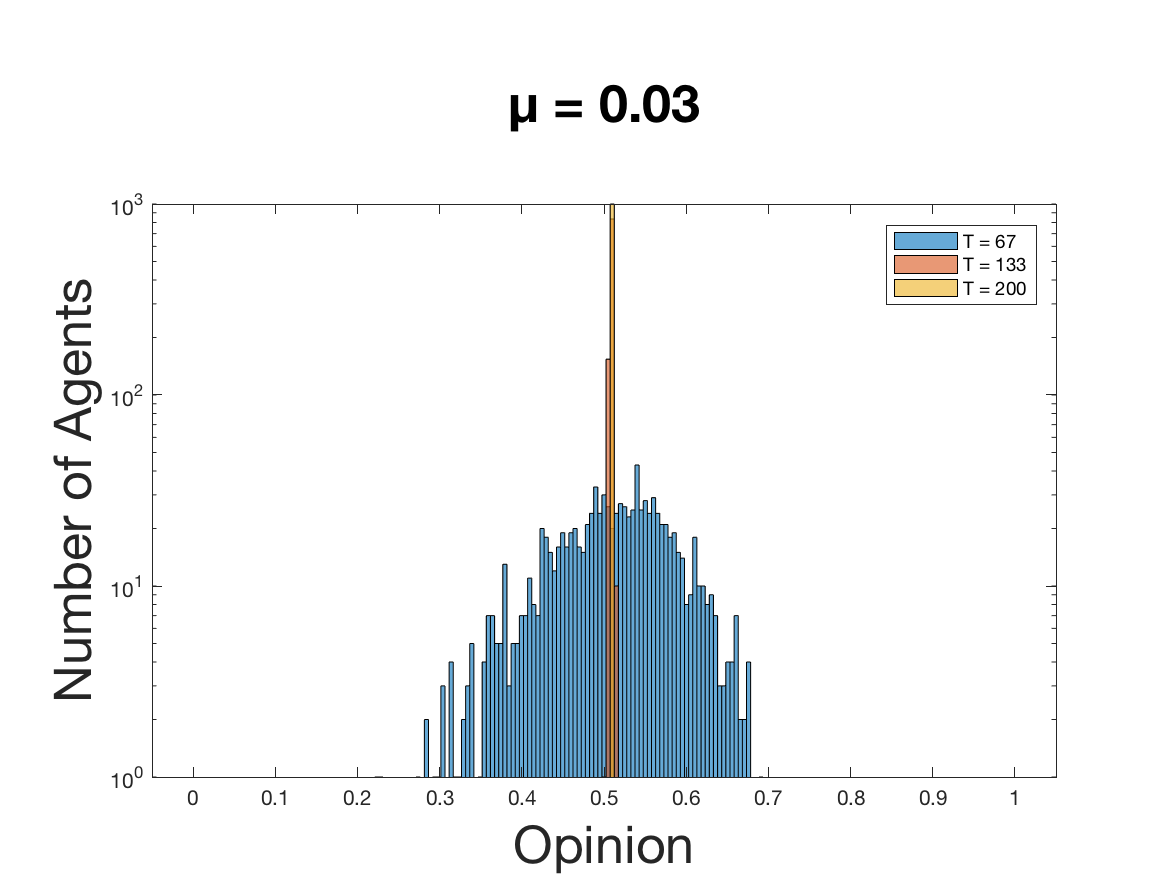
\includegraphics[width=\linewidth]{gen_plot_2017121813322472200e+01.png}
\endminipage\hfill
\minipage{0.5\textwidth}
  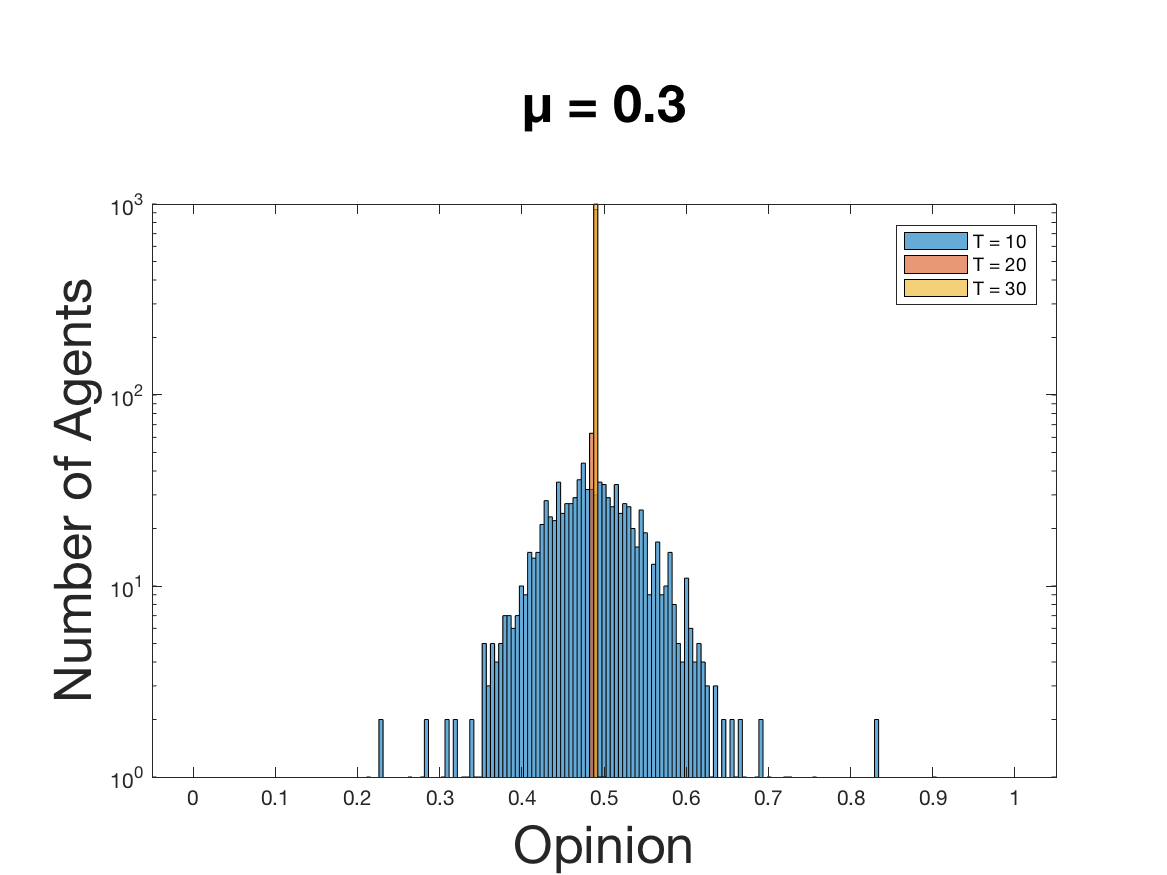
\includegraphics[width=\linewidth]{gen_plot_2017121813324648428e+00.png}
\endminipage
\caption{Opinion distribution for different times in a society \textbf{without extremists} for a given $\mu$ of 0.03 or 0.3. We fixed the number of society agents $N = 1000$ and the threshold $u = 0.3$}
\label{fig:muwithoutextremists}
\end{figure}


\subsection{Cluster building}
According to \cite{Minor}, such a society of N agents with random uniform distributed opinions $x_i$ in [0,1] will converge to a common opinion around 0.5 if the communicating interval $u$ of agents communicating with each other is big enough, more precise if $u>0.3$. This was repeated and shown in figure \ref{fig:uwithoutextremists}. \\

\begin{figure}[!htb]
\center
  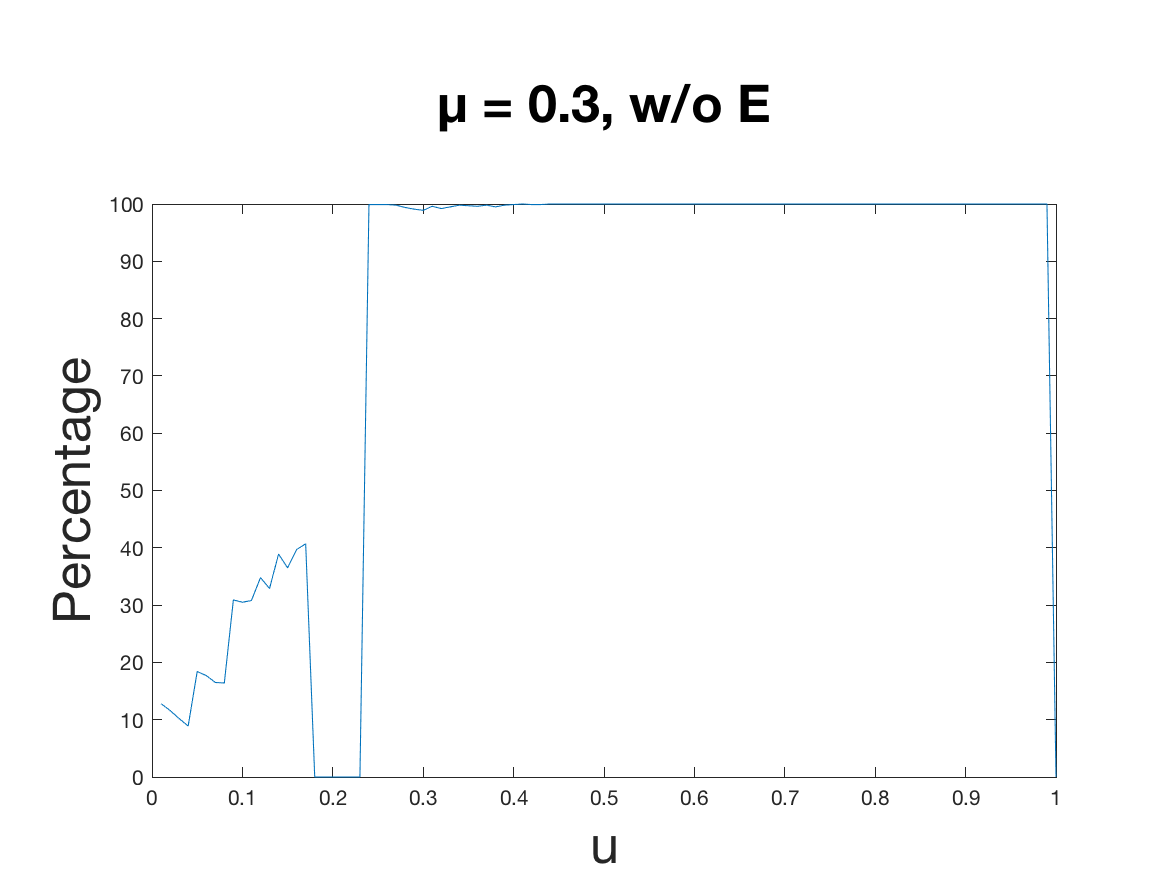
\includegraphics[width=0.7\linewidth]{gen_plot_intervall_2017121816214390840e+01.png}
  \caption{Percentage of agents in central cluster between 0.45 and 0.55 when varying $u$}
  \label{fig:uwithoutextremists}
\end{figure}

In case $u = 0$, there is no opinion interaction between the agents and the uniform distribution of the opinions gives us the percentage $\frac{|0.45-0.50|}{1} = 10\%$. For values of $u$ between 0.18 and 0.22 we see that almost no opinions are between 0.45 and 0.55. This corresponds to the fact that the opinions converge against two opinions that are around 0.25 and 0.75, shown in \cite{Minor}. If $u > 0.28$ we see almost 100\% in this cluster. This is the main result of this chapter and is defined as the convergence against a common opinion around 0.5.

\section{A world with extremists}
The society model described above is being extended to a society with extreme opinion individuals who can influence the agents. We carry on to vary different parameters in this society model.

\subsection{The "new" parameter \texorpdfstring{$\mu$}{TEXT}}
In the case of a society without extremists, $\mu$ was a measure of convergence. However, it did not have an influence on the final result. If a small $\mu$ was chosen, the number of time steps T could be increased accordingly to get the same result of convergence (See Chapter 4.1). \\*
While varying the values of $\mu$ in a society with extremists, $\mu$ does not only influence the speed of convergence, but also the spread of opinions. If a small $\mu$ is chosen, thus the natural convergence is slow, this leads to more agents with extreme opinions, compared to a high $\mu$. See figure \ref{fig:muwithextremists} and \ref{fig:muwithextremists2} and see that there are more extremists in the case of a small $\mu$, different as in figure  \ref{fig:muwithoutextremists}.

\begin{figure}[!htb]
\minipage{0.5\textwidth}
  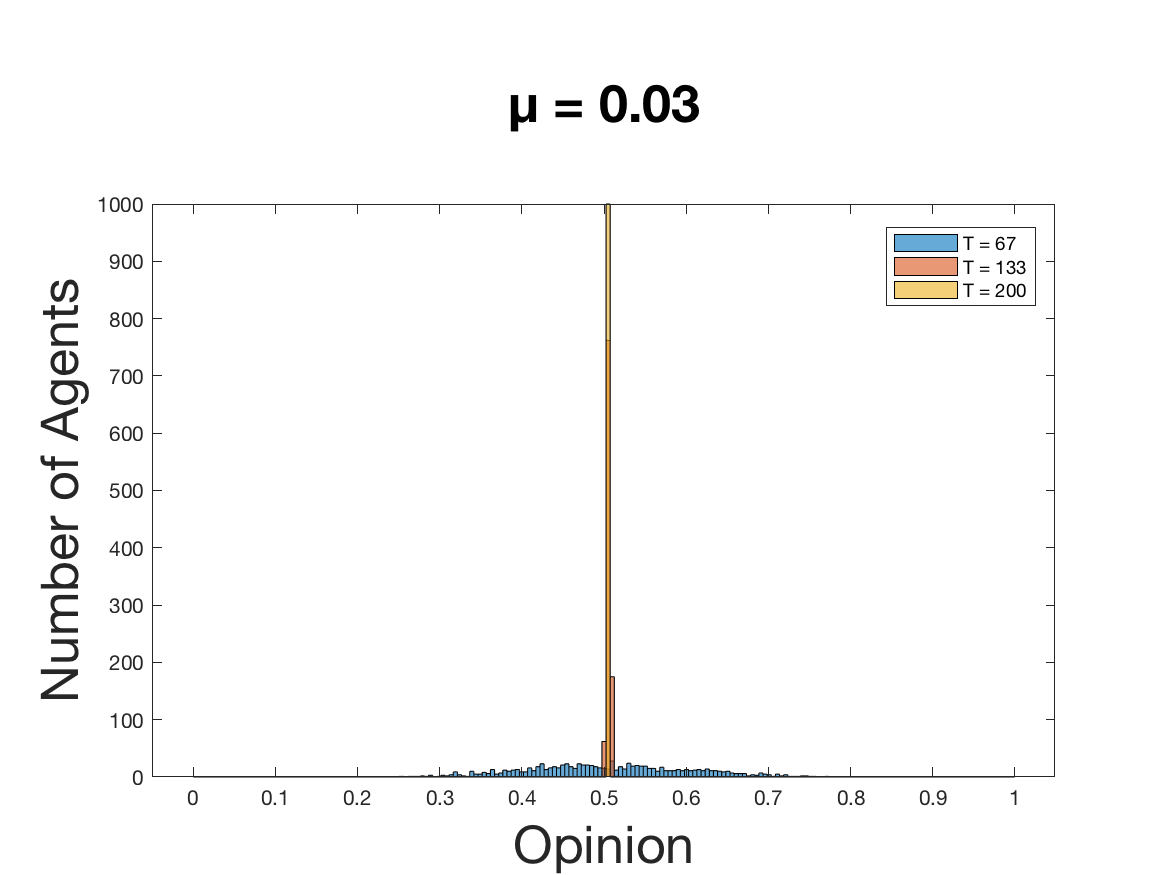
\includegraphics[width=\linewidth]{gen_plot_2017121418225017531e+01.png}
\endminipage\hfill
\minipage{0.5\textwidth}
  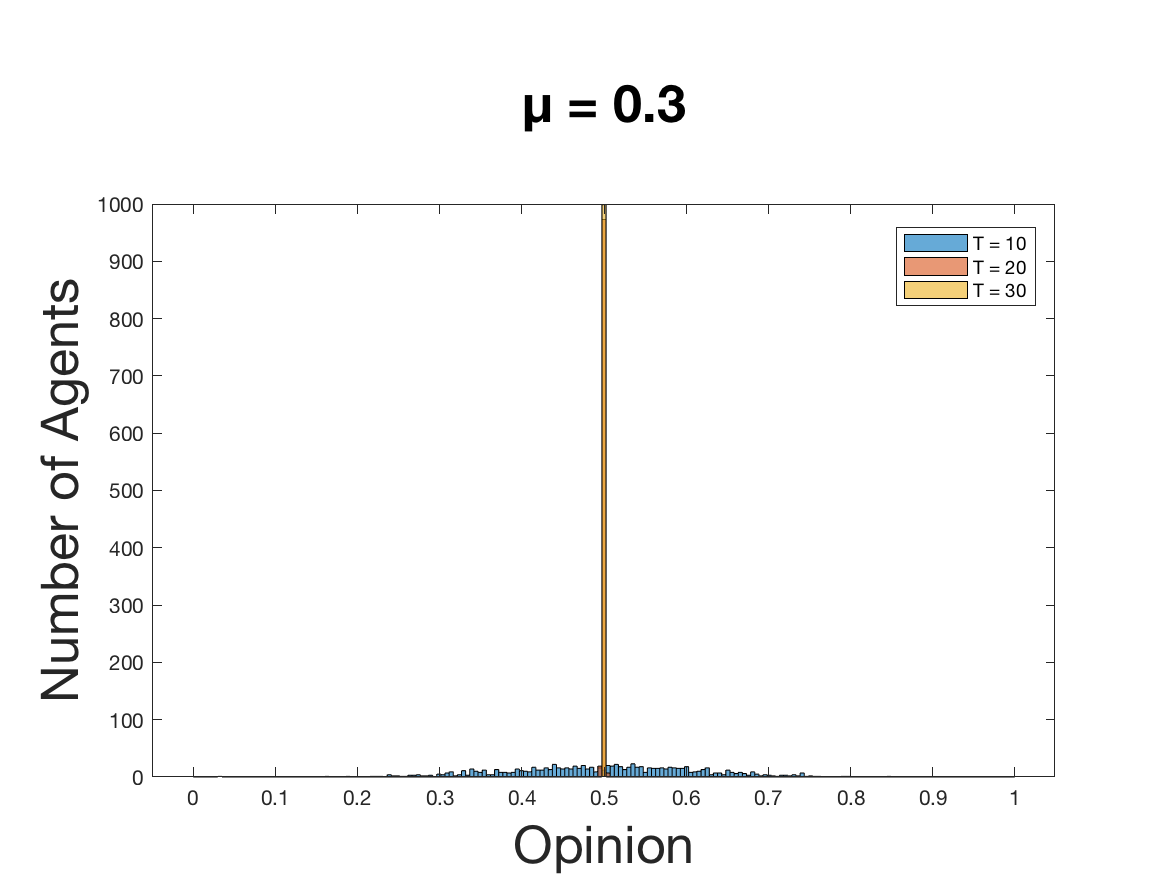
\includegraphics[width=\linewidth]{gen_plot_2017121418225354249e+01.png}
\endminipage
\caption{Opinion distribution for different times in a society \textbf{with extremists} for a given $\mu$ of 0.03 or 0.3. We fixed the number of society agents $N = 1000$ and the threshold $u = 0.3$ for $n_{conv}$ = 10}
\label{fig:muwithextremists}
\end{figure}

This can be explained as follows: If the natural convergence is slow, more time steps are needed to get to the stationary state. But the extremists influence is independent of $\mu$. Therefore, if the natural influence is small, the extremists have more time to grasp agents with opinions in the interval accessible to the the agents who could pull them to the average opinion cluster at $x$ = 0.5.

\begin{figure}[!htb]
\minipage{0.5\textwidth}
  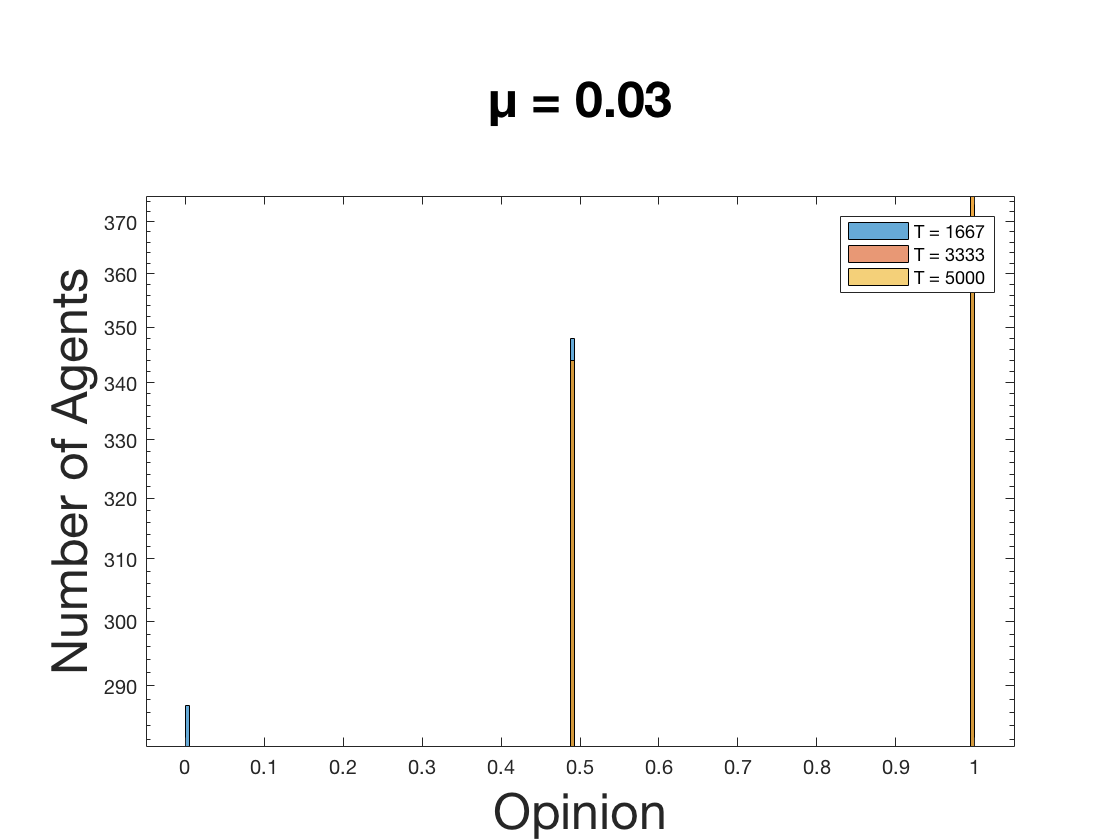
\includegraphics[width=\linewidth]{gen_plot_geil_klein_mu.png}
\endminipage\hfill
\minipage{0.5\textwidth}
  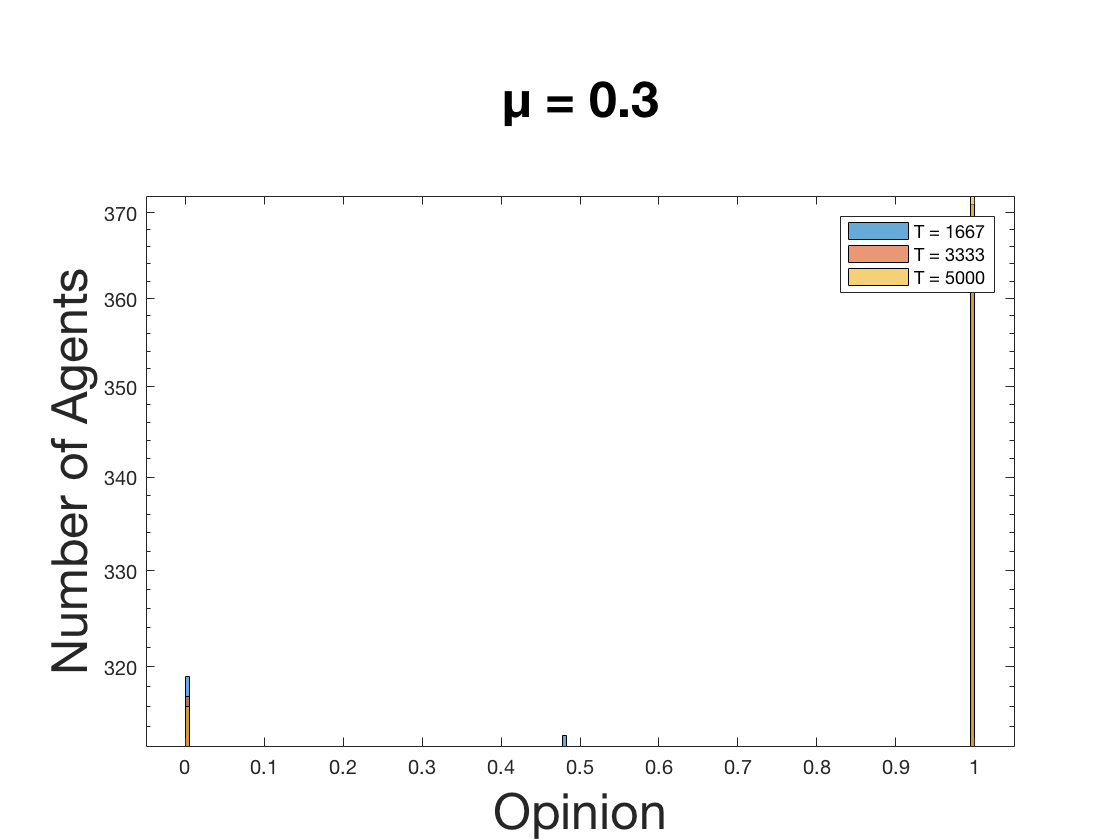
\includegraphics[width=\linewidth]{gen_plot_geil_gross_mu.png}
\endminipage
\caption{Opinion distribution for different times in a society \textbf{with extremists} for a given $\mu$ of 0.03 or 0.3. We fixed the number of society agents $N = 1000$ and the threshold $u = 0.3$ for $n_{conv} = 100$}
\label{fig:muwithextremists2}
\end{figure}


\subsection{The interval of influence}
Next, the interval of influence $infop$ is varied. Concretely, the range of people influenced by the extremists with opinion $x=0$ is in [0, infop] and by the extremists with opinion $x=1$ is in [1-infop, 1]. We vary infop from 0 to 0.5. 

The results can be seen in figure \ref{fig:varinfop}. We see that the convergence with this set of parameters is amazingly stable until we come close to $infop = 0.5$. Further, the number of convinced agents, defined by $n_{conv}$ and controlled by varying p, has a small influence for small $infop$, but at exactly 0.5 a higher $p$ leads to more extremists.

If a low number of extremists ($p \leq 20$) takes influence on our society, it is important for them to reach almost every opinion even in the middle. Otherwise we always see a strong cluster around the opinion 0.5. Note that for $infop = 0.5$ we reach all opinions which will lead to a situation where all agents have extreme opinions for T running against infinity.

\begin{figure}[!htb]
\begin{subfigure}[t]{\textwidth}
\minipage{0.32\textwidth}
  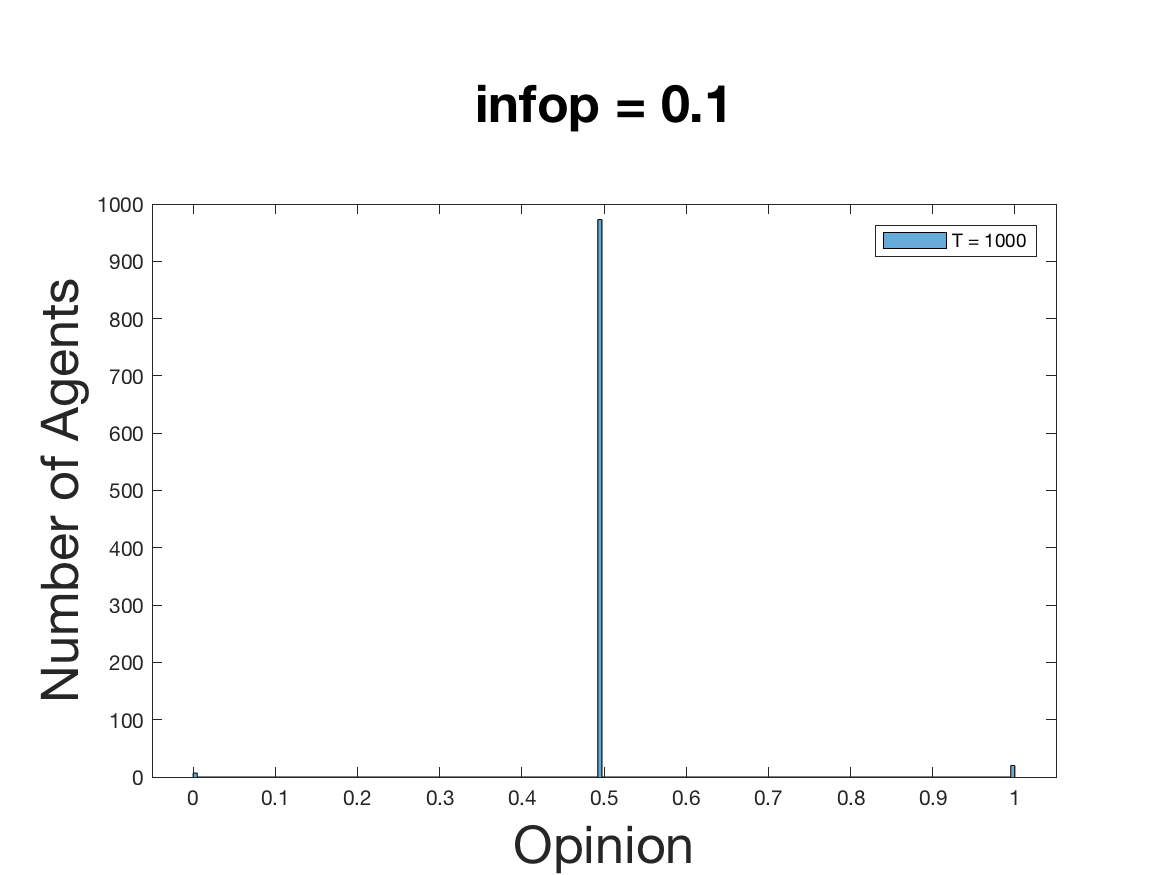
\includegraphics[width=\linewidth]{p_5/gen_plot_201712171365061157e+01.png}
\endminipage\hfill
\minipage{0.32\textwidth}
  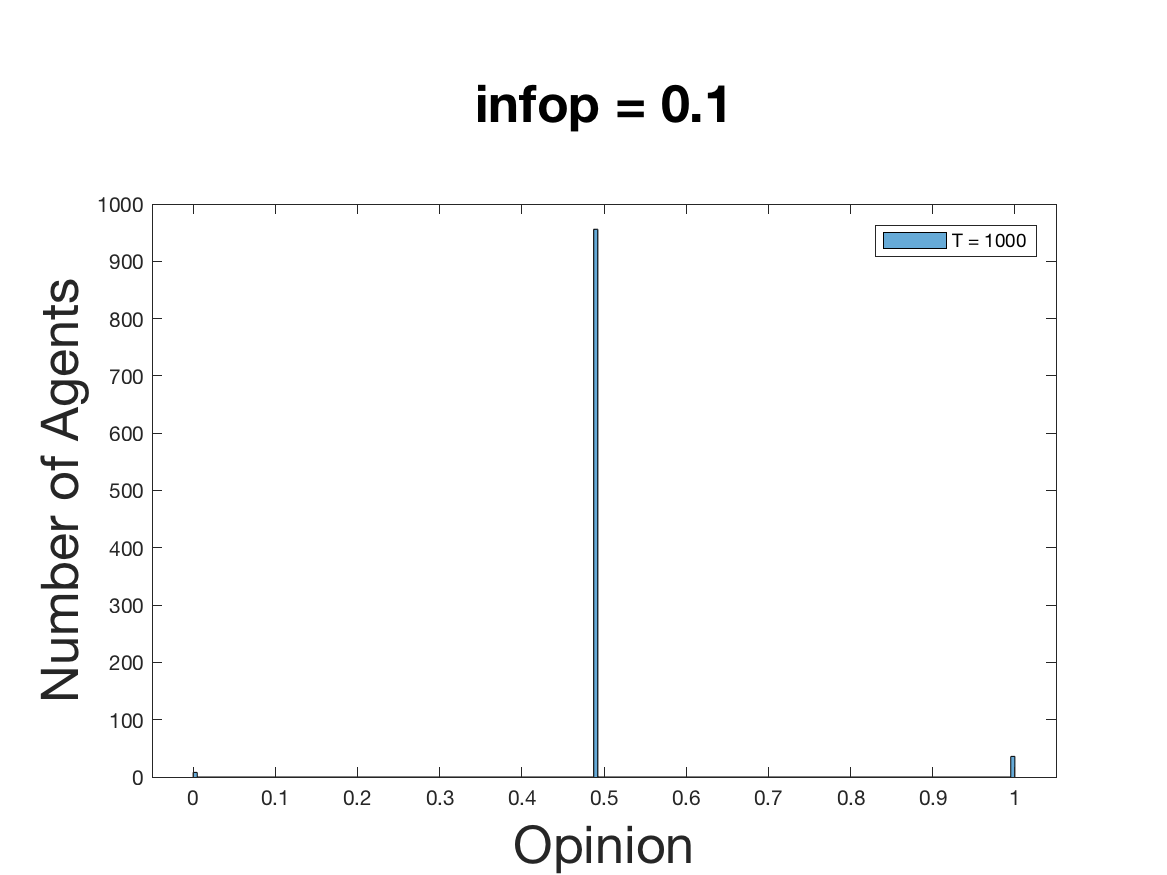
\includegraphics[width=\linewidth]{p_10/gen_plot_2017121712593240672e+01.png}
\endminipage\hfill
\minipage{0.32\textwidth}
  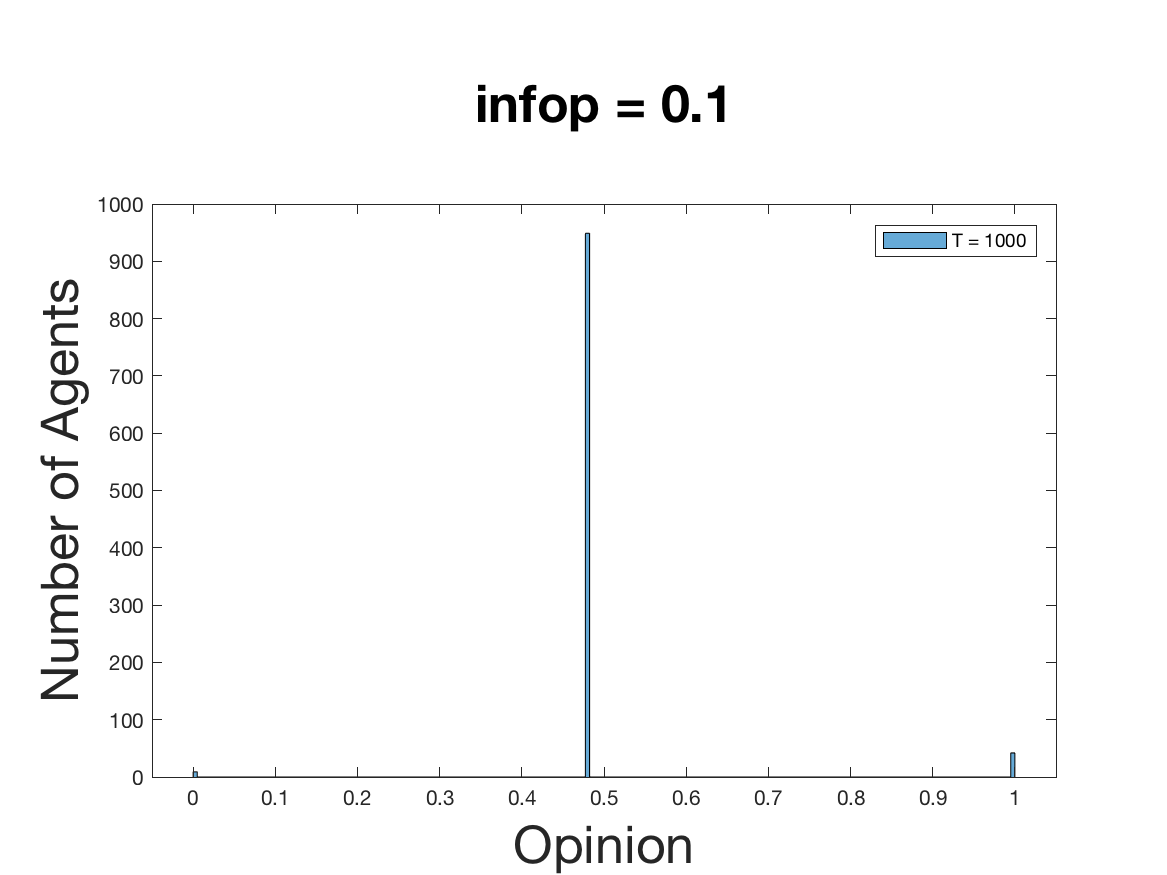
\includegraphics[width=\linewidth]{p_20/gen_plot_201712171361168753e+01.png}
\endminipage
\end{subfigure}


\begin{subfigure}[!htb]{\textwidth}
\minipage{0.32\textwidth}
  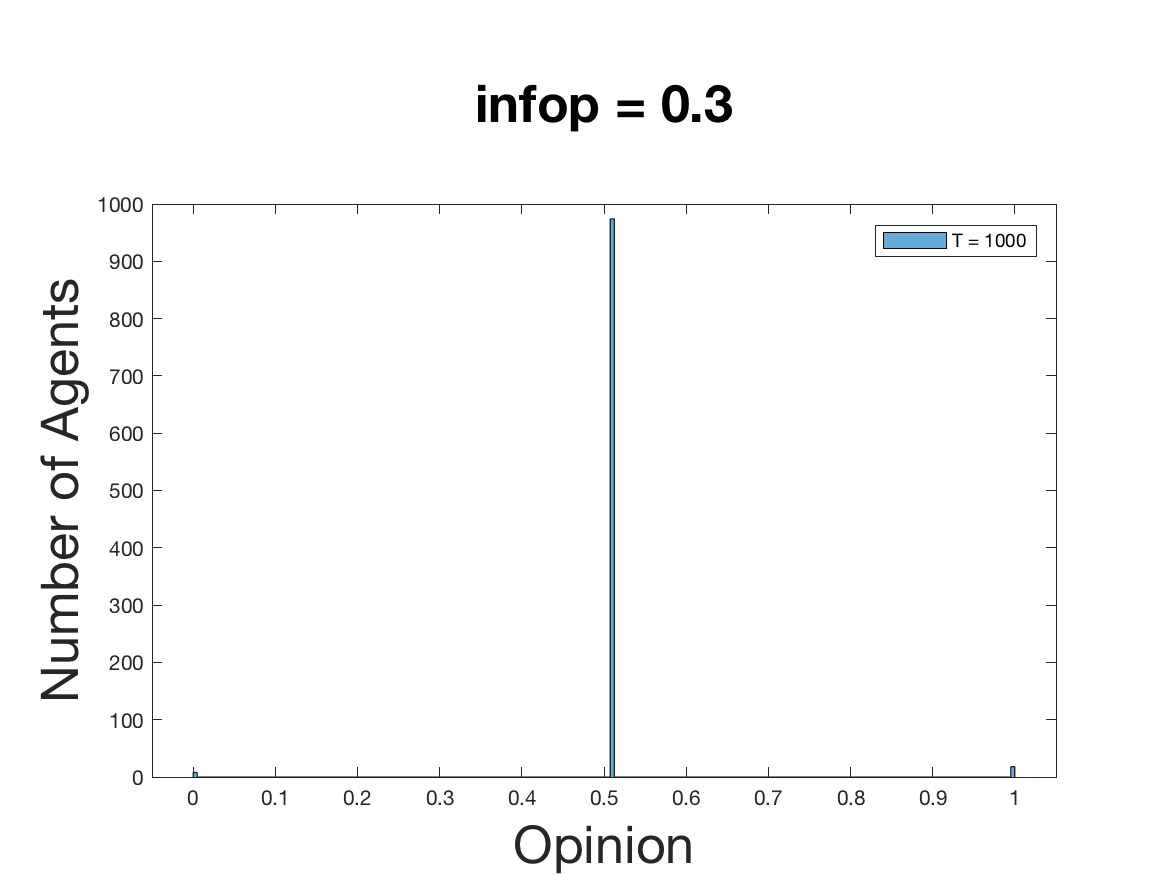
\includegraphics[width=\linewidth]{p_5/gen_plot_201712171365491110e+01.png}
\endminipage\hfill
\minipage{0.32\textwidth}
  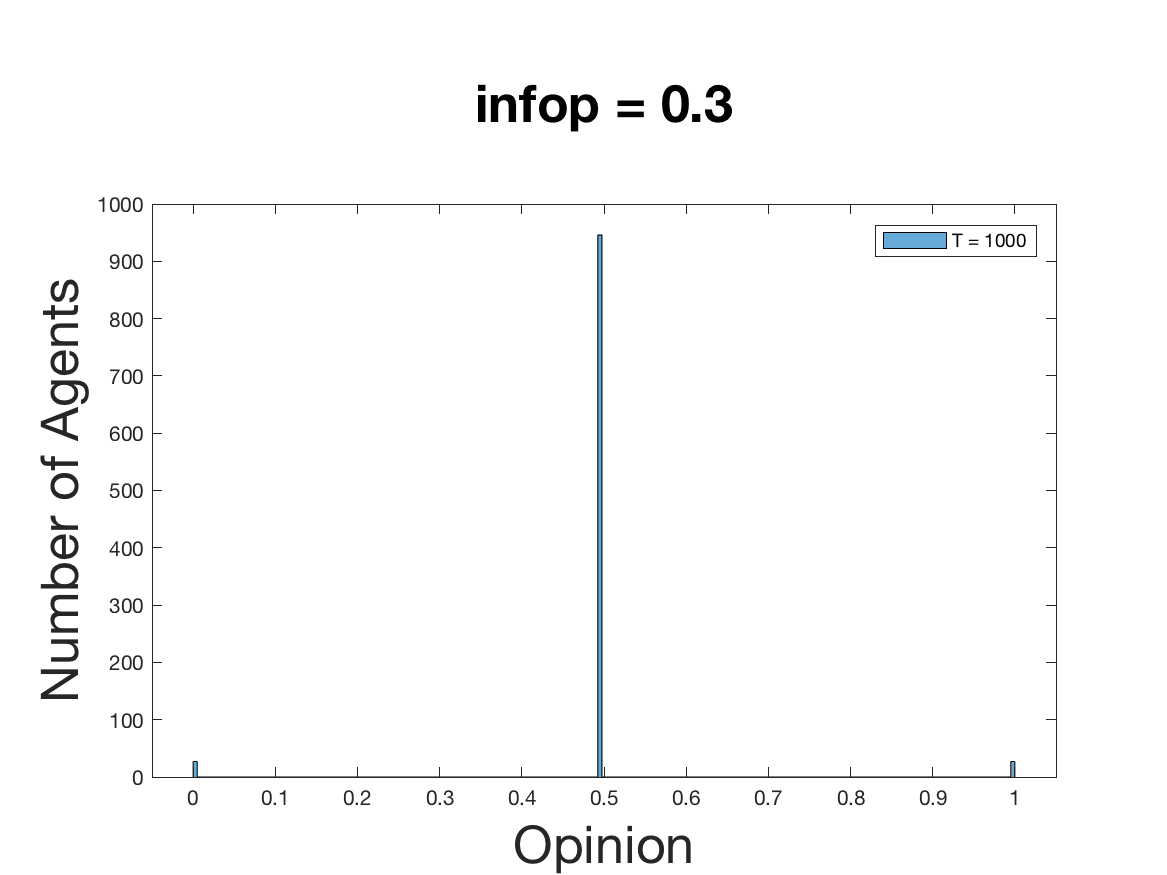
\includegraphics[width=\linewidth]{p_10/gen_plot_2017121712593647221e+01.png}
\endminipage\hfill
\minipage{0.32\textwidth}
  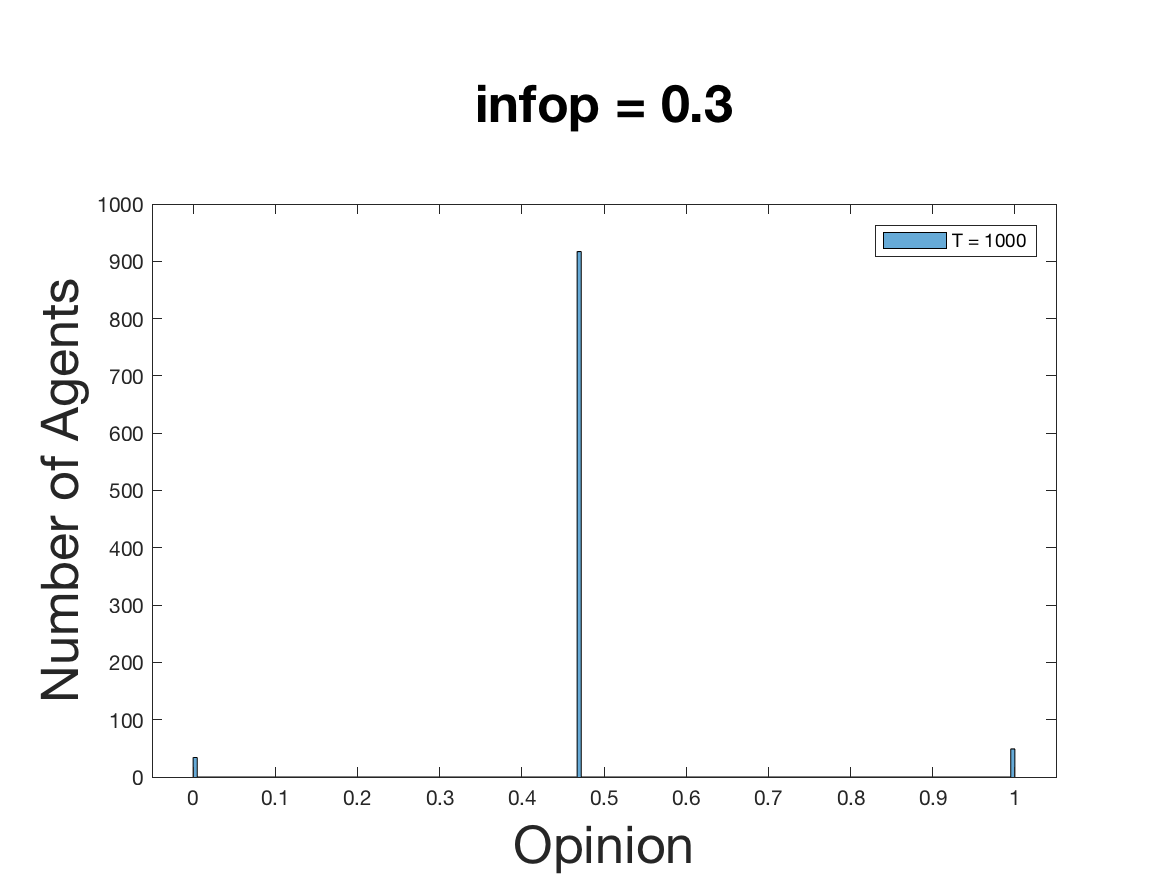
\includegraphics[width=\linewidth]{p_20/gen_plot_201712171361653386e+01.png}
\endminipage
\end{subfigure}


\begin{subfigure}[!htb]{\textwidth}
\minipage{0.32\textwidth}
  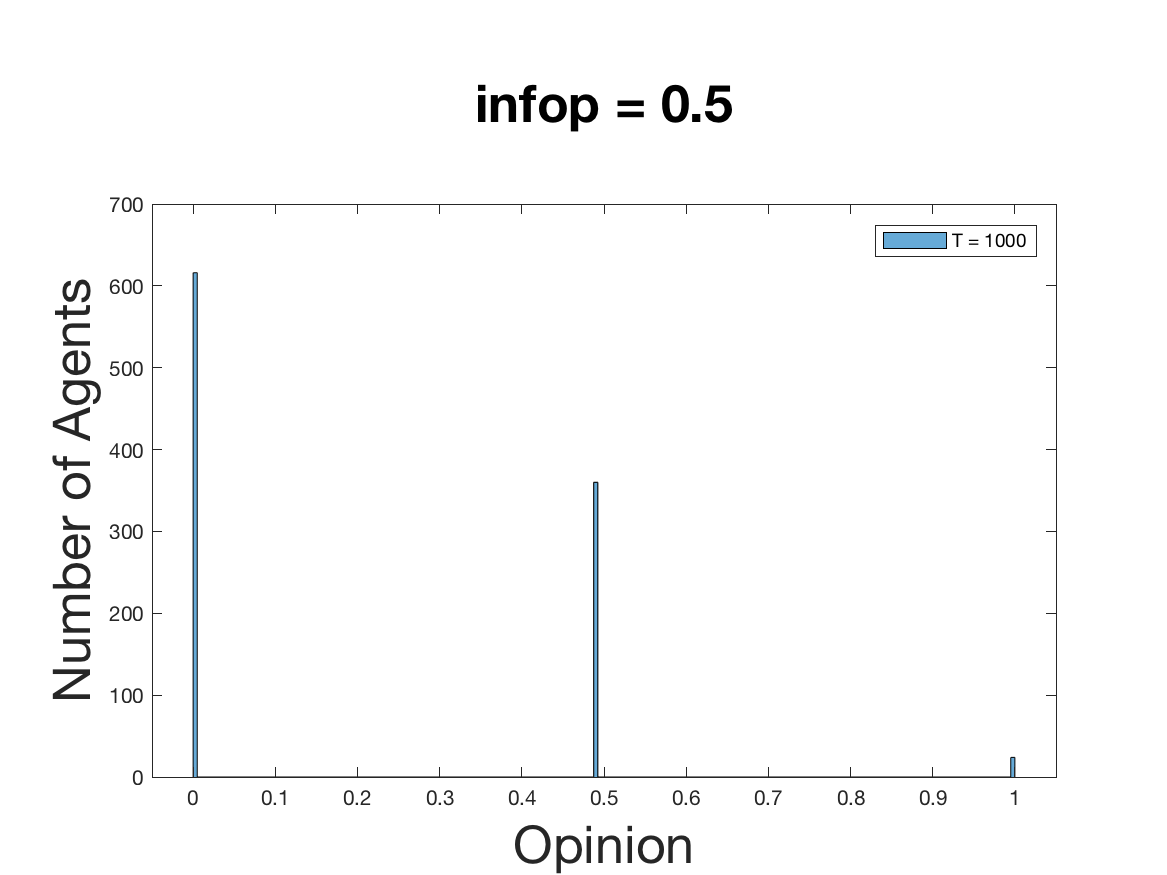
\includegraphics[width=\linewidth]{p_5/gen_plot_201712171365898973e+01.png}
\endminipage\hfill
\minipage{0.32\textwidth}
  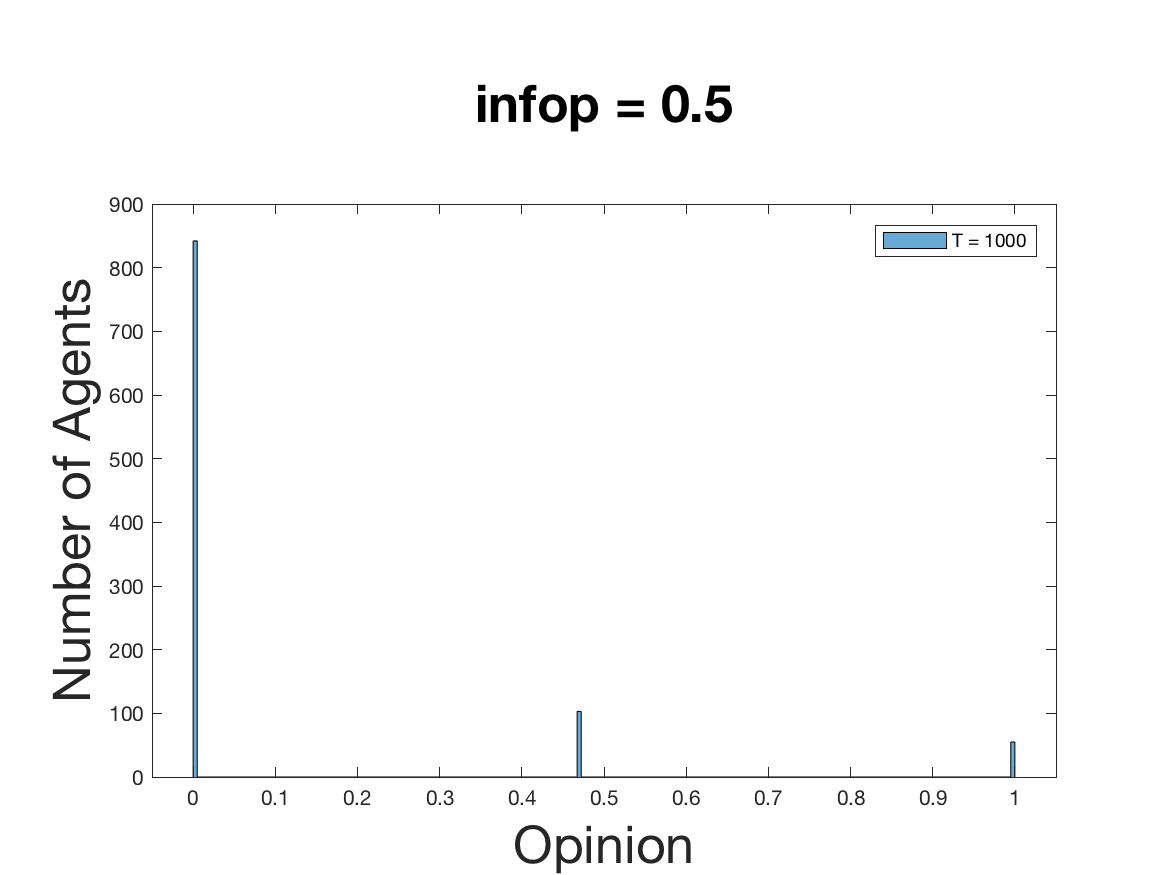
\includegraphics[width=\linewidth]{p_10/gen_plot_2017121712596271176e+00.png}
\endminipage\hfill
\minipage{0.32\textwidth}
  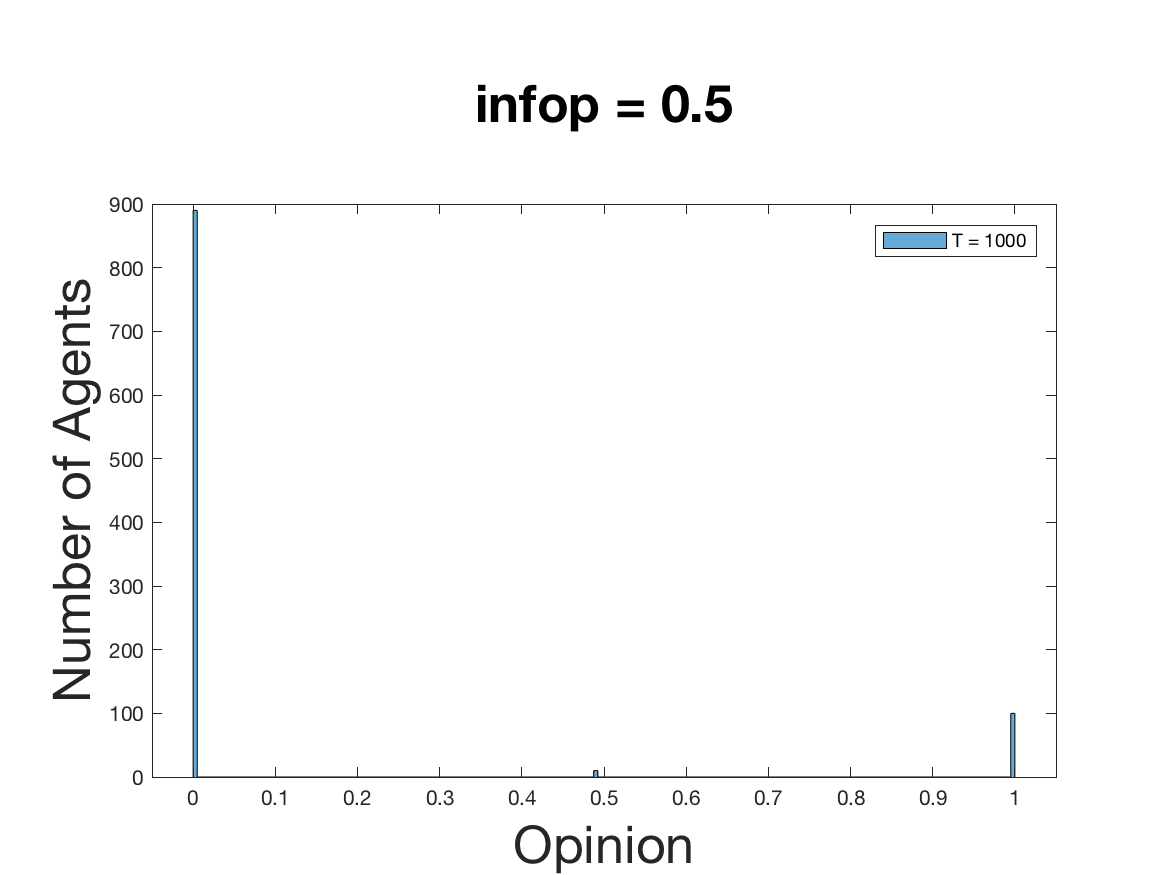
\includegraphics[width=\linewidth]{p_20/gen_plot_201712171362013207e+01.png}
\endminipage
\end{subfigure}

\caption{Opinion spread for different $infop$ for p = 5, 10 and 20 (from left to right). We fixed $N = 1000$, $\mu = 0.3$ and $u = 0.32$.}
\label{fig:varinfop}
\end{figure}



\subsection{The power of convincing}
We fix $\mu = 0.1$ and $u = 0.32$ to be sure that in the case of a society without extremists we would see a common convergence of opinions to 0.5. The extremists are inserted with $infop = 0.3$. We examine the development of the number of extreme opinions. More precise we measure the percentage of the opinions in the intervals $x \in [0, 0.1] \cap [0.9, 1]$. \\*
For simplicity we fix $n = 1$ and $\kappa = 0.2$ and vary the number of influence-able people $p \in [0,P]$. One can calculate the final parameter for the amount of influenced agents simply with $n_{conv} = n\cdot\kappa\cdot p$. \\*

\begin{figure}[!htb]
\center

  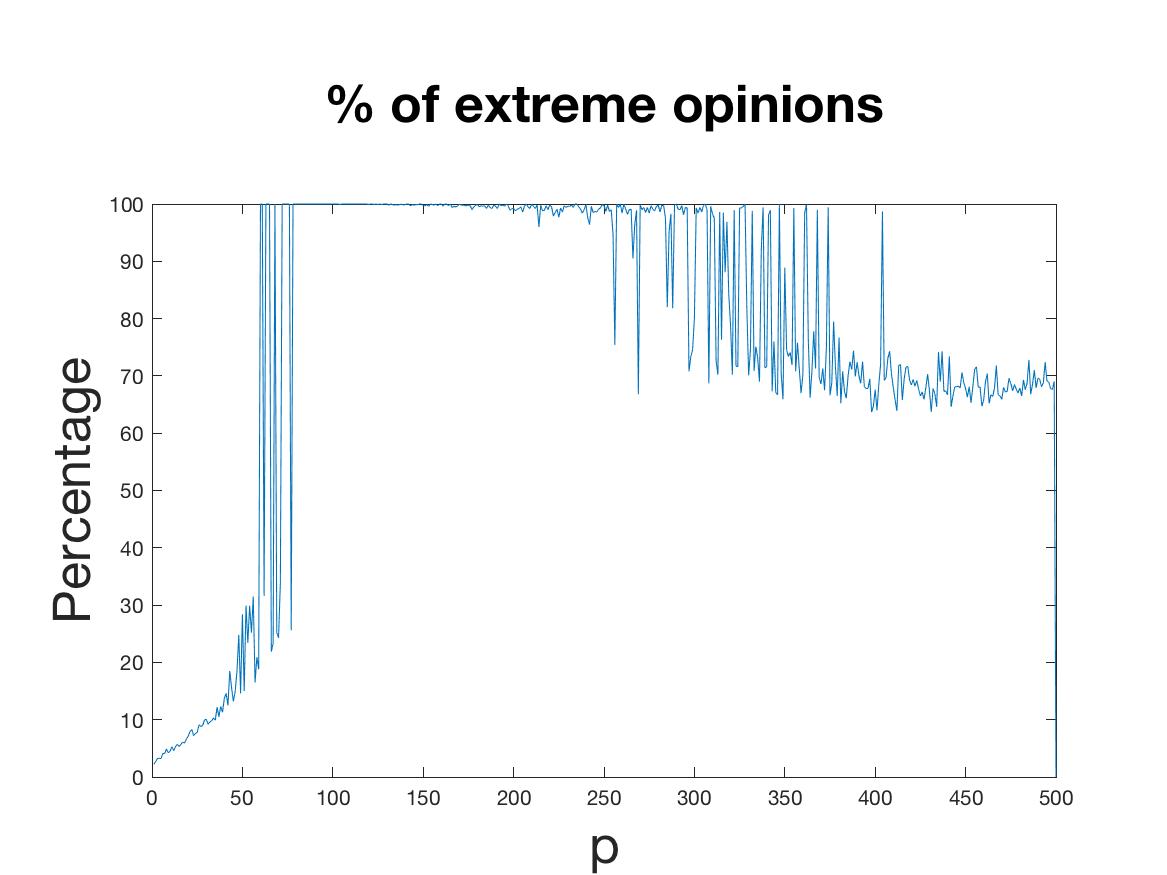
\includegraphics[width=0.6\linewidth]{gen_plot_intervall_201712182172720605e+01.png}
  \caption{Fraction of extreme opinions in $[0, 0.1] \cap [0.9, 1]$ for convinced agents $\propto$ $p$}
  \label{fig:varynconv}
\end{figure}

Figure \ref{fig:varynconv} shows the result of the described measurement. For $p < 50$ we see a proportional relation to the  percentage of extreme opinions. It is obvious that a higher convincing rate should provoke more extreme opinions. For $50 < p < 250$ we see a jump and the extremists manage to convince the whole society. An interesting case is given again for $p > 250$. The percentage of the extreme opinion goes down again. This corresponds to the fact that they destroy "bridges". They are so strong that they collect all agents in their range defined by $infop$ within a few time steps. It stays a rest in the middle that converges again to 0.5.

The interesting numbers are $p = 50$ and $p = 250$. They define the range in which the extremists are able to use $\mu$ to their advantage and are strong enough to collect all agents even if they cannot reach all agents directly (see chapter 4.2).


\section{Discussion}
The challenge of the simulation was to keep track of which parameters were to be varied in the society with extremists compared to the society wihtout. We managed to reproduce the effects explained in the paper. The fact that Laguna found converging opinions for $u>0.3$ and we found converging opinions already for $u>0.24$ is unexplained. However, we assumed that we implemented the code like Laguna.

It was very interesting to see the change of the parameter $\mu$ in the second society compared to the first. It was further interesting to see that a variation of the interval of influence $infop$ did not make a big difference on the result up to the point where $infop$ comes close to the value 0.5. In chapter 5.3, we also found a interval for strength of the extremists. If the number of influencable agents was increased, first the proportion of extreme opinions increased linearly, then jumped to 100$\%$ and decreased again for a very high number of influencable agents.\\*


\section{Summary and Outlook}
Until now we considered only symmetric random distributions and symmetric distribution of extremists. We could have also 
What is gonna happen if this will be asymmetric? What would be the interpretation? What is interesting in these cases?


If we do no Gaussian distribtion: a normal distribution is a sensible alternative opinion distribution where 0.5 is the main stream opinion and other opinions are spreaded around the main stream distribution. Sigma would be measure for 'how far' the other opinions are spreaded from the main stream opinion.

Higher N corresponds to other bridge effects. (see chapter 5.3)


%\section{References}
\begin{thebibliography}{99}
\bibitem{Coevolutions} Peter Holme and M. E. J. Newman. \textit{Nonequilibrium phase transition in the coevolution of networks and opinions}. arXiv:physics/0603023v3, 9 March 2006.

\bibitem{Minor} M. F. Laguna, Guillermo Abramson, and Damian H. Zanette. \textit{Minorities in a Model for Opinion Formation}. Wiley Periodicals, Inc., Vol. 9, No.4, 5 January 2004

\end{thebibliography} 


\end{document}

